\documentclass[12pt,letterpaper]{article}
\usepackage{amsmath,amsthm,amsfonts,amssymb,amscd}
\usepackage{listings}
\usepackage{color}
\usepackage{MnSymbol,wasysym}
\usepackage{caption}
\usepackage{subcaption}

\definecolor{dkgreen}{rgb}{0,0.6,0}
\definecolor{gray}{rgb}{0.5,0.5,0.5}
\definecolor{mauve}{rgb}{0.58,0,0.82}

\lstset{%frame=tb,
  language=Bash,
  aboveskip=3mm,
  belowskip=3mm,
  showstringspaces=false,
  columns=flexible,
  basicstyle={\small\ttfamily},
  numbers=none,
  numberstyle=\tiny\color{gray},
  keywordstyle=\color{blue},
  commentstyle=\color{dkgreen},
  stringstyle=\color{mauve},
  breaklines=true,
  breakatwhitespace=true
  tabsize=3
}


\usepackage{hyperref}
\usepackage{graphicx}
\usepackage{enumerate}
\usepackage{fancyhdr}
\usepackage{mathrsfs}
\usepackage[margin=3cm]{geometry}
\setlength{\parindent}{0.0in}
\setlength{\parskip}{0.05in}

% Edit these as appropriate
\newcommand\course{CS595}
\newcommand\semester{FAll 2013}     
\newcommand\hwnum{6}
\newcommand\yourname{Mohamed Aturban}
\newcommand\login{maturban}

\newenvironment{answer}[1]{
  \subsubsection*{Problem #1}
}

\pagestyle{fancyplain}
\headheight 40pt
\lhead{\yourname\ (\login)\\\course\ --- \semester}
\chead{\textbf{\Large Assignment \hwnum}}
\rhead{\today}
\headsep 40pt

\begin{document}

All files mentioned in this document should be uploaded into the {\it github} repository.

\begin{answer}{1}

R script, {\it rcode.r}, has been written to work on Karate Club graph and try predicating same result. I have used the idea of Girvan-Newman algorithm, explained in our class (week 7 slides -- Graph Analysis), This algorithm is depending on calculating the edge betweennees of all edges in the graph and then remove the one that has the maximum value. Repeating this several times will lead the graph to split into different regions. The following is a brief description of how the algorithm works:

\begin{itemize}
\item Read the graph vertices and edges from \url{http://igraph.sourceforge.net/karate.net}.
\item Compute betweenness values of all edges using:

\begin{lstlisting}
			edge.betweenness( graph )
\end{lstlisting}

\item Remove the edge that has the maximum betweenness.
\item Stop if the graph is split into two different clusters. This can be done by checking the value of {\it clusters( graph )[ 'no' ] }.
\item if {\it clusters( graph )[ 'no' ]} is still equal to one, repeat again from step 2.
\end{itemize}

Let me show the algorithm output into two different format:

\begin{enumerate}
  \item Text format:
	after each iteration, the edge, which has the maximum betweenness value, will be printed on the screen along with its betweenness value:

\begin{lstlisting}
	Edges will be deleted in the following order :
 	1  ->  32   -- Betweenness =  68.454304029304
	1  ->  3    -- Betweenness =  62.757375957376
	1  ->  9    -- Betweenness =  83.0110106432357
	14 ->  34   -- Betweenness =  82.1695725842785
	20 ->  34   -- Betweenness =  123.46625041625
	3  ->  33   -- Betweenness =  100.372222222222
	2  ->  31   -- Betweenness =  139.182683982684
	2  ->  3    -- Betweenness =  109.25
	3  ->  4    -- Betweenness =  107.666666666667
	3  ->  14   -- Betweenness =  142.75
	3  ->  8    -- Betweenness =  285
\end{lstlisting}	
	    
  
  
  
  \item Graphs: 
  a graph, in R, will be drawn on the screen after each iteration indicating which of the edges has been deleted. see the following figures:
\end{enumerate} 


\begin{figure}
\centering
\begin{subfigure}{.5\textwidth}
  \centering
  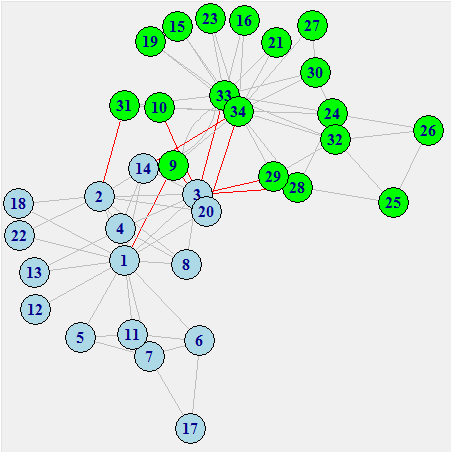
\includegraphics[width=.9\linewidth]{132}
  \caption{After removing 1 $->$ 32}
  \label{fig:sub1}
\end{subfigure}%
\begin{subfigure}{.5\textwidth}
  \centering
  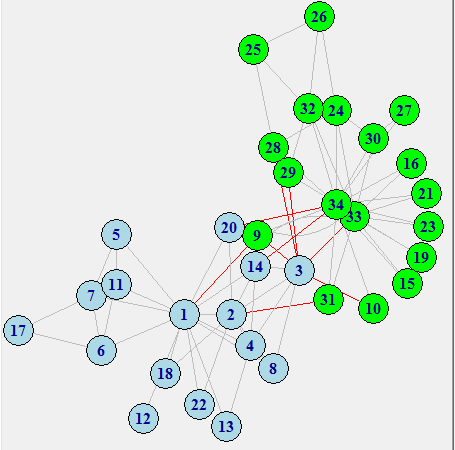
\includegraphics[width=.9\linewidth]{13}
  \caption{After removing 1 $->$ 3}
  \label{fig:sub2}
\end{subfigure}
\caption{First two algorithm iterations}
\label{fig:test}
\end{figure}


\begin{figure}
\centering
\begin{subfigure}{.5\textwidth}
  \centering
  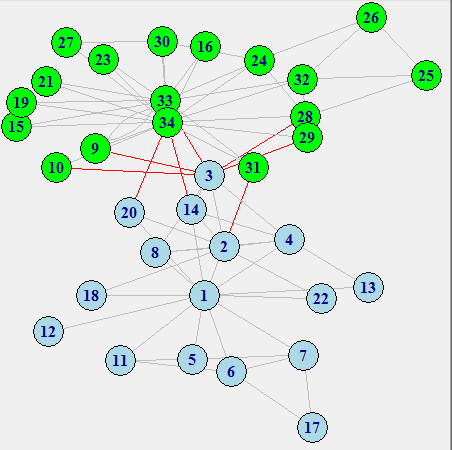
\includegraphics[width=.9\linewidth]{19}
  \caption{After removing 1 $->$ 9}
  \label{fig:sub1}
\end{subfigure}%
\begin{subfigure}{.5\textwidth}
  \centering
  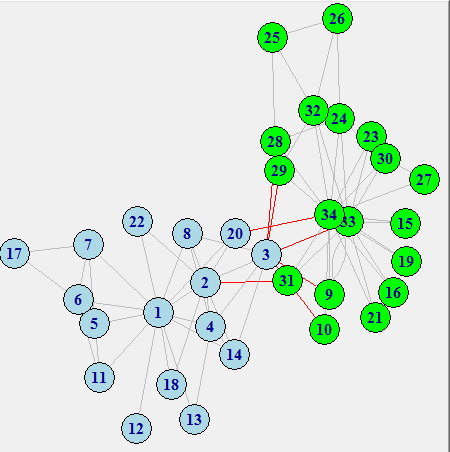
\includegraphics[width=.9\linewidth]{1434}
  \caption{After removing 14 $->$ 34}
  \label{fig:sub2}
\end{subfigure}
\caption{Third and forth iterations}
\label{fig:test}
\end{figure}


\begin{figure}
\centering
\begin{subfigure}{.5\textwidth}
  \centering
  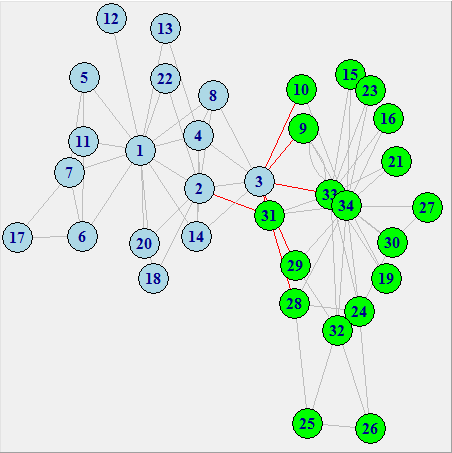
\includegraphics[width=.9\linewidth]{2034}
  \caption{After removing 20 $->$ 34}
  \label{fig:sub1}
\end{subfigure}%
\begin{subfigure}{.5\textwidth}
  \centering
  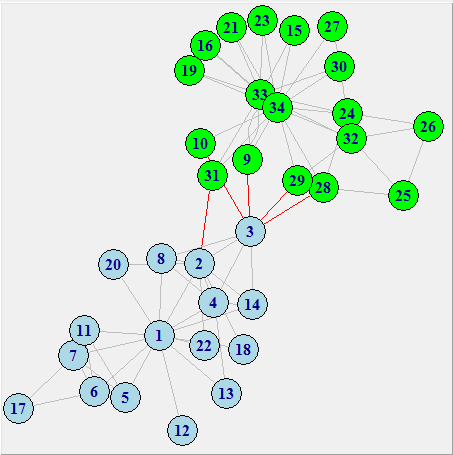
\includegraphics[width=.9\linewidth]{333}
  \caption{After removing 3 $->$ 33}
  \label{fig:sub2}
\end{subfigure}
\caption{Fifth and sixth iterations}
\label{fig:test}
\end{figure}

\begin{figure}
\centering
\begin{subfigure}{.5\textwidth}
  \centering
  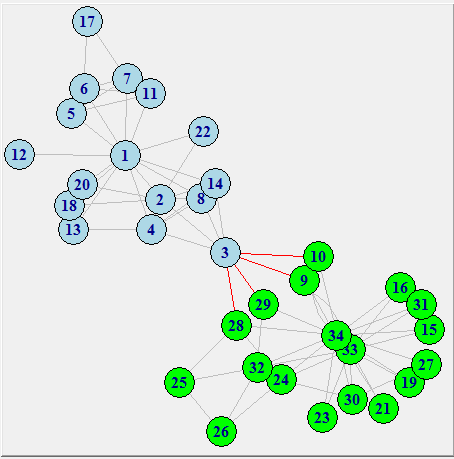
\includegraphics[width=.9\linewidth]{231}
  \caption{After removing 2 $->$ 31}
  \label{fig:sub1}
\end{subfigure}%
\begin{subfigure}{.5\textwidth}
  \centering
  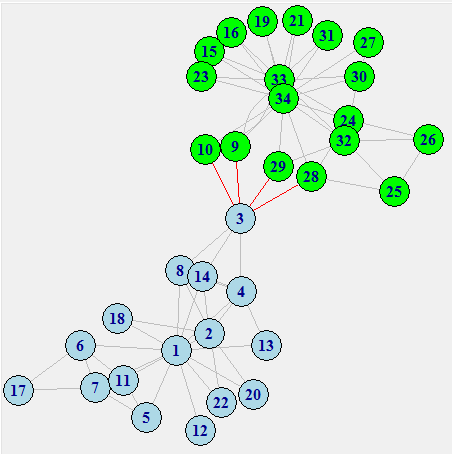
\includegraphics[width=.9\linewidth]{23}
  \caption{After removing 2 $->$ 3}
  \label{fig:sub2}
\end{subfigure}
\caption{Iteration number seven and eight}
\label{fig:test}
\end{figure}

\begin{figure}
\centering
\begin{subfigure}{.5\textwidth}
  \centering
  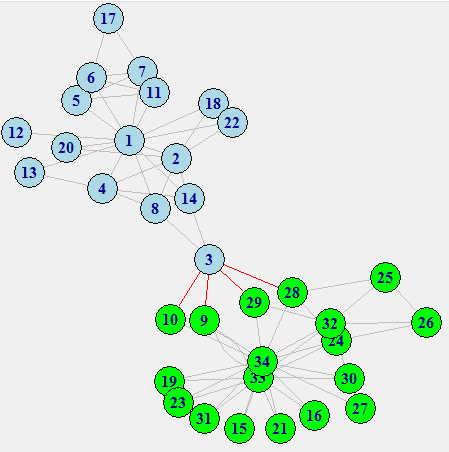
\includegraphics[width=.9\linewidth]{34}
  \caption{After removing 3 $->$ 4}
  \label{fig:sub1}
\end{subfigure}%
\begin{subfigure}{.5\textwidth}
  \centering
  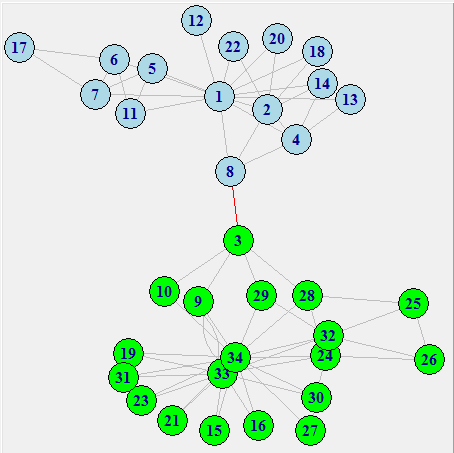
\includegraphics[width=.9\linewidth]{314}
  \caption{After removing 3 $->$ 14}
  \label{fig:sub2}
\end{subfigure}
\caption{Ninth and tenth Iterations}
\label{fig:test}
\end{figure}

\begin{figure}[ht!]
\centering
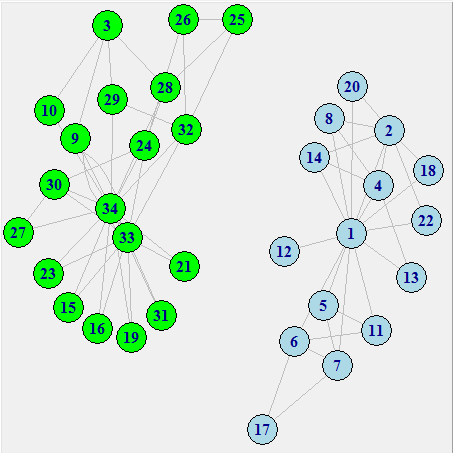
\includegraphics[scale=0.9]{38}
\caption{After removing 3 $->$ 8: Final Graph is split into two clusters}
\label{overflow}
\end{figure}


In conclusion, the result obtained from our algorithm is really close to the Karate Club graph. The only difference here is that node no. 3 has decided to change her mind and move to the other party. 

\end{answer}



\begin{answer}{2}

This depends on which nodes will join new groups or move between that existing groups, but, in general, I believe that even by adding 2 or 3 different new group, node no. 1 and 34 will remain strong and keep their communities (groups) alive since they are connecting to most of other nodes. If more groups are established, then, I have no idea how the new graph will look like.

\end{answer}

\end{document}
